\section{Inledning}
Jag har gjort en filhanterar som visualiserar alla filer och mappar i 3D med hjälp av OpenGL. Inspirationen till detta projekt var bland annat FSN (File System Navigator) som gjordes av SGI för IRIX systemen och FSV(File System Visualizer) som är en remake av FSN på Linux, se figur~\ref{fig:fsn}. En annan inspiration var det lite modernare TDFSB som även visar upp bilder och filmer i 3D världen, se figur~\ref{fig:tdfsb}. 

\begin{center}
\begin{figure}[H]
    \centering
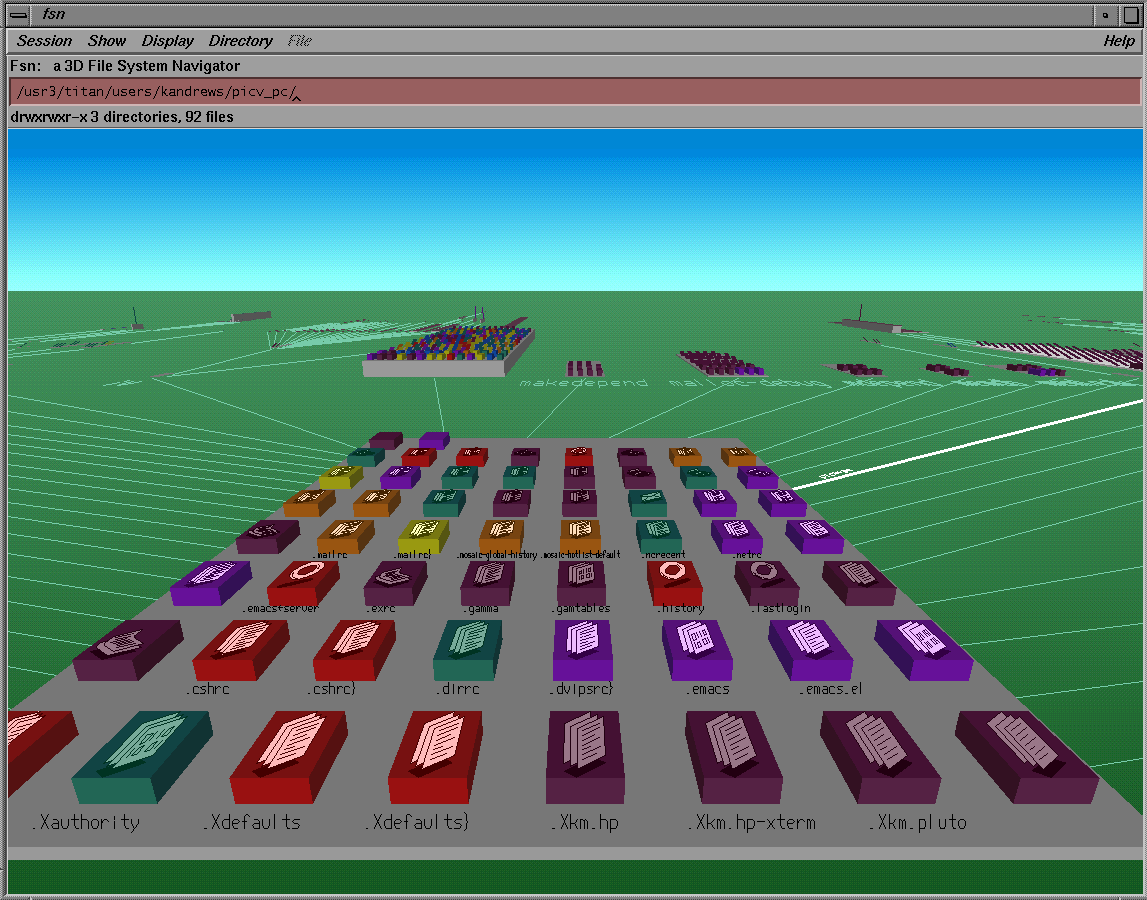
\includegraphics[width=8cm]{../grafik/fsn1.png}
\caption{FSN.}
\label{fig:fsn}
\end{figure}
\end{center}

\begin{center}
\begin{figure}[H]
    \centering
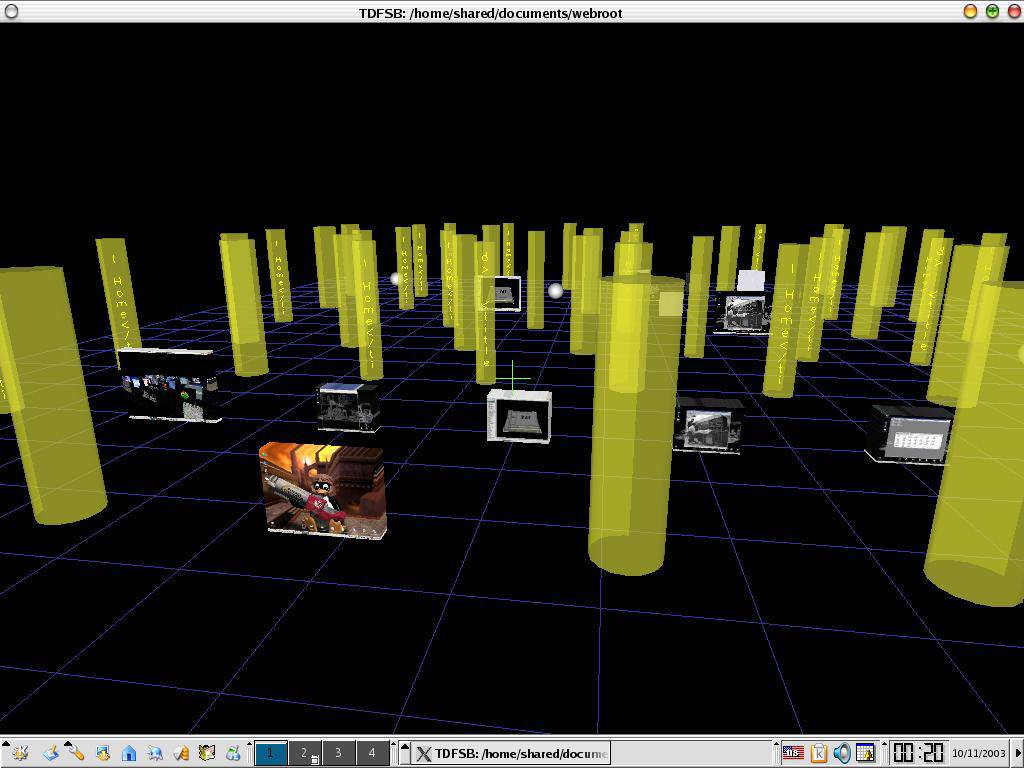
\includegraphics[width=8cm]{../grafik/tdfsb.jpg}
\caption{TDFSB.}
\label{fig:tdfsb}
\end{figure}
\end{center}

De ursprungliga obligatoriska kraven för produkten var följande:
\begin{LIPSkravlista}
\LIPSkrav{Original}{Alla filer ska representeras av block med någon textur på, är det en bild så ska bilden användas som textur}{1}

\LIPSkrav{Original}{Alla mappar ska representeras av block med någon textur}{1}
\LIPSkrav{Original}{Alla mappar och filer i en mapp ska vara placerade på en platta med en textur}{1}
\LIPSkrav{Original}{Ljussättningen ska ske med en Phong-shader}{1}
\LIPSkrav{Original}{Alla block ska ha skuggor}{1}
\LIPSkrav{Original}{Navigeringen ska vara first person där piltangenterna styr x och z koordinaterna och musen styr kameren i ett sfäriskt koordinatsystem}{1}
\LIPSkrav{Original}{Man ska inte kunna gå igenom filerna(collisions detection)}{1}
\LIPSkrav{Original}{Du ska kunna gå in i en mapp så transporteras du till den nya mappen)}{1}
\LIPSkrav{Original}{Du ska kunna klicka på en fil/mapp och få upp alla möjliga alternativ såsom radera, öppna...)}{1}
\LIPSkrav{Original}{Om du raderar en fil ska övriga filer ordna sig så det inte är några luckor någonstans}{1}
\LIPSkrav{Original}{Skydome ska finnas}{1}
\LIPSkrav{Original}{Endast Linux kommer stödjas}{1}
\end{LIPSkravlista}


och de ej obligatoriska kraven var följande:
\begin{LIPSkravlista}
\LIPSkrav{Original}{Du ska kunna få upp en terminal i filhanteraren}{2}
\LIPSkrav{Original}{Du ska kunna klicka på en mapp och sedan få upp en portal som du kan se in i mappen genom}{2}
\LIPSkrav{Original}{När du raderar en fil ska den explodera}{2}
\LIPSkrav{Original}{Innehåller en mapp många filer/mappar ska frustum culling användas för att minimera beräkningar}{2}
\LIPSkrav{Original}{Mapparnas texturer ska vara den ikon filen som operativsystemet använder med transparens, då ska renderingsordningen och vara korrekt}{2}
\end{LIPSkravlista}
Under projektets gång gick de obligatoriska kraven igenom en modifikation på grund av att projektet tog längre tid än vad jag trodde samt att en del inte riktigt passade in. Krav 5 togs bort på grund av tidsbrist, krav 6 gjordes om så att användaren bara navigerade i XZ planet då detta passade mycket bättre samt en del förenklingar kunde göras. Krav 9 togs bort då en terminal ansågs vara mycket enklare att implementera så all modifikation av filsystemet görs via den. Inga av de ej obligatorska kraven uppfylldes på grund av tidsbrist. I figur~\ref{fig:tmbtrf} kan man se resultatet. 
\begin{center}
\begin{figure}[H]
    \centering
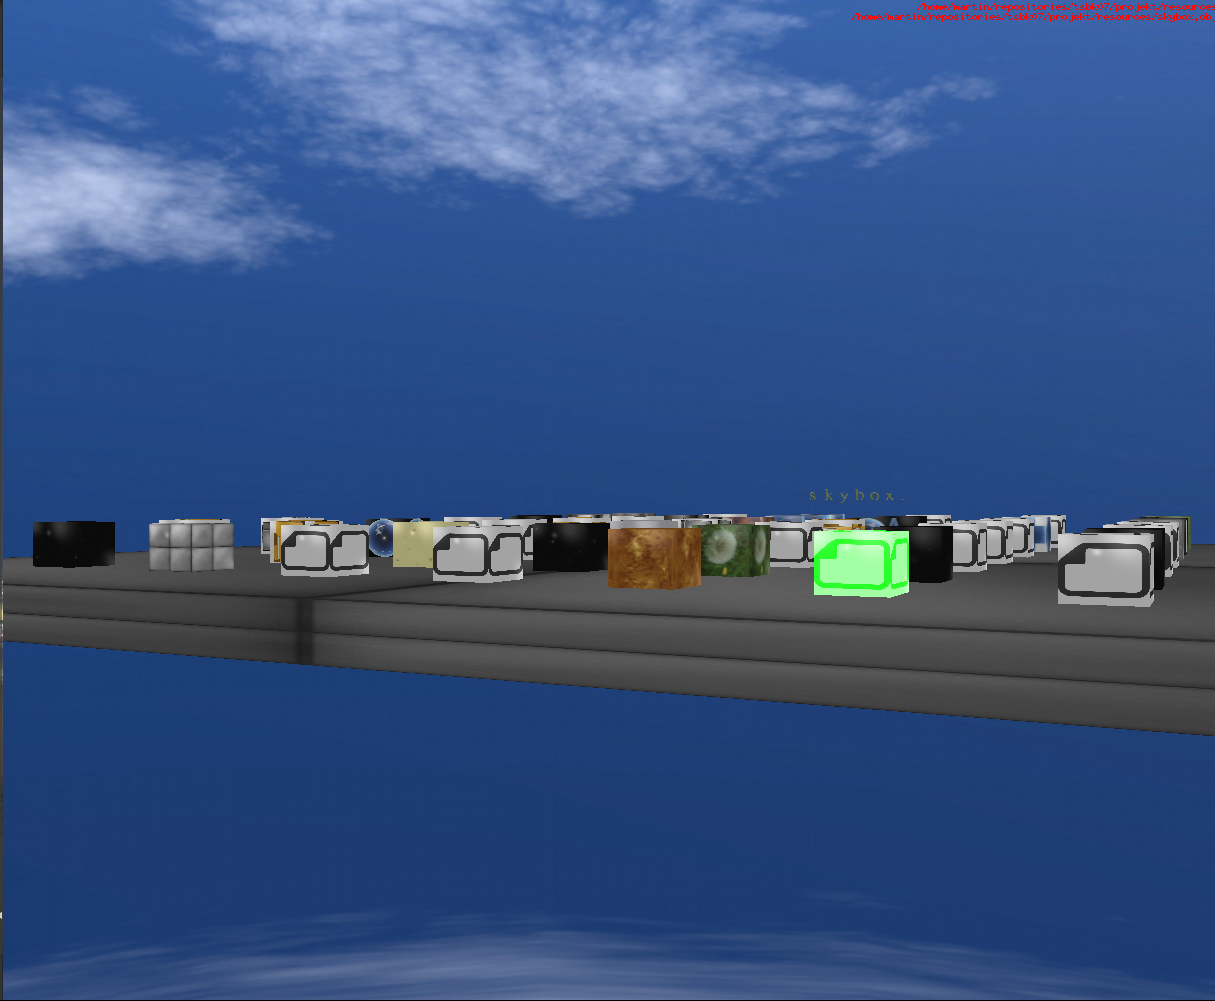
\includegraphics[width=8cm]{../grafik/tmbtrf.png}
\caption{TMBTRF.}
\label{fig:tmbtrf}
\end{figure}
\end{center}
